% Copyright (c) 2019 Bochen Tan
% Public domain.
%本模板的宗旨是尽量绿色,不需要附加安装任何东西。
%按照教务部下发的WORD说明文档格式,下简称“说明”
%没有封面和评阅表,这两部分请直接在Cover&ReviewTable.doc中写再输出pdf拼到一起
%doc小改动:封面校徽和文字替换为了高清版本,“题目:”和中文题目对齐,中英文题目分在了表的两行
%doc小改动:插入了两个白页,使得连续打印的时候封面和表格都在奇数页
%正文部分改动:在每一页下方中央加了页码,因为说明中页眉不分奇偶页,所以页码就都在中央吧
%不含自动的参考文献,因为说明中参考文献格式不典型,请手动输入或自行写程序
%在Windows或Linux下渲染出字体更接近说明,Mac OS上字体不太一样
%有警告\headheight is too small,fancyhdr的上距离有点小,似乎问题不大

\documentclass[UTF8,openany,AutoFakeBold,AutoFakeSlant,cs4size]{ctexbook}
%openany 使一章可以从偶数页开始,因为说明中每一章并没有只能从奇数页开始,虽然这是常理
%AutoFakeBold 和 AutoFakeSlant 因为 CJK 里没有真正的加粗和倾斜,如果额外字体则效果更好
%cs4size 因为要求主题是小四号字

\usepackage[a4paper,left=3.18cm,right=3.18cm,top=2.54cm,bottom=2.54cm]{geometry}
%office中正常页边距



\usepackage{amsmath}
\usepackage{bm}
\usepackage{amsfonts}
\usepackage{enumerate}
\usepackage{fancyhdr}



\usepackage{cite}
\newcommand{\upcite}[1]{\textsuperscript{\cite{#1}}} %引用在右上角



\usepackage{multirow,booktabs,makecell}
\usepackage{graphicx}
\usepackage[font=small,labelsep=space]{caption} %五号,宋体/Time new roman
\renewcommand{\thetable}{\arabic{table}} %表格和图片编号不分章节,直接1,2,3 ...
\renewcommand{\thefigure}{\arabic{figure}}
\renewcommand{\theequation}{\arabic{chapter}.\arabic{equation}} %公式标签 章.公式(均为阿拉伯数字)



\usepackage{tocloft} %自定义目录,说明中没有明确规定,和WORD自动生成目录格式一致

%“全文目录”四个字的格式
\renewcommand\cftbeforetoctitleskip{0pt}
\renewcommand\cftaftertoctitleskip{0pt}
\renewcommand\cfttoctitlefont{\bfseries\heiti\zihao{2}}

\renewcommand\cftchapfont{\heiti\normalsize} %黑体小四
\renewcommand\cftchapdotsep{\cftdotsep} %有点连到页码,点间距不确定,待改
\renewcommand\cftchappagefont{\songti\normalsize} %宋体小四页码
\renewcommand\cftbeforechapskip{0pt}

%1. 第一级 五号宋体,缩进两个字符,页码一致
\renewcommand\cftsecfont{\songti\small}
\renewcommand\cftsecpagefont{\songti\small}
\renewcommand\cftsecaftersnum{.} %一级目录号后加点
\renewcommand\cftsecindent{2em}
\renewcommand\cftbeforesecskip{0pt}

%1.1 第二级 五号宋体,缩进四个字符,页码一致
\renewcommand\cftsubsecfont{\songti\small}
\renewcommand\cftsubsecpagefont{\songti\small}
\renewcommand\cftsubsecindent{4em}
\renewcommand\cftbeforesubsecskip{0pt}

%1.1.1 第二级 五号宋体,缩进四个字符,页码一致
\renewcommand\cftsubsubsecfont{\songti\small}
\renewcommand\cftsubsubsecpagefont{\songti\small}
\renewcommand\cftsubsubsecindent{4em}
\renewcommand\cftbeforesubsubsecskip{0pt}



\usepackage{titlesec}%自定义章节标题
\CTEXsetup[format={\bfseries\center\heiti\zihao{2}},beforeskip=0pt]{chapter}
%第一章  绪论(二号、黑体) beforeskip为上方垂直距离看起来还比说明偏大,待改

\setcounter{tocdepth}{3}
\setcounter{secnumdepth}{3}
%使目录中有三级标题,即subsubsection

\renewcommand\thesection{\arabic{section}} % 使得不显示章名,只显示节名
\titleformat{\section}
{\raggedright\zihao{3}\bfseries\songti}
{\thesection.\quad}
{0pt}
{}%1. 第一级(三号、宋体/Time new roman、加粗)

\titleformat{\subsection}
{\raggedright\bfseries\zihao{4}\songti}
{\thesubsection\quad}
{0pt}
{}%1.1 第二级(四号,宋体/Time new roman,加粗)

\titleformat{\subsubsection}
{\raggedright\bfseries\zihao{-4}\songti}
{\thesubsubsection\quad}
{0pt}
{}%1.1.1 第三级(小四,宋体/Time new roman,加粗)




% 封面依赖的宏包
\usepackage{xcoffins} % 用于设计封面格式
\usepackage{xcolor}
\usepackage{xeCJK} % 用于引入楷体
\usepackage{soul} % 用于设置下划线宽度
\setul{}{2pt}
\setmainfont{Times New Roman} % Times New Roman 作为默认英文字体
% 引入楷体,请改成自己系统里对应的名字
\setCJKfamilyfont{kaiti}[AutoFakeBold=1.5]{楷体}
\newcommand{\kaiti}{\CJKfamily{kaiti}}

% 评阅表依赖的宏包
\usepackage{float}
\usepackage{array}




\title{}
\author{}
\date{}
\begin{document}

% 封面中需要修改的内容直接在此处更改即可
\newcommand{\chineseTitle}{三维模型最优二维视图生成方法研究}
\newcommand{\englishTitle}{Synthesizing best 2D views of 3D models}
\newcommand{\name}{黄道吉}
\newcommand{\studentID}{1600017857}
\newcommand{\school}{元培学院}
\newcommand{\major}{计算机科学与技术}
\newcommand{\advisor}{连宙辉}
% 插入封面
% 声明需要的Coffin
\NewCoffin \result
\NewCoffin \topBox
\NewCoffin \badge
\NewCoffin \pku
\NewCoffin \headingText
\NewCoffin \titleText
\NewCoffin \chineseTitleText
\NewCoffin \englishTitleText
\NewCoffin \nameText
\NewCoffin \studentIDText
\NewCoffin \schoolText
\NewCoffin \majorText
\NewCoffin \advisorText
\NewCoffin \dateText


% 各个Coffin的内容
\SetHorizontalCoffin \result {}
\SetHorizontalCoffin \topBox {\color{white} \rule{210mm}{41mm}}
\SetHorizontalCoffin \badge {
\includegraphics[width=20.6mm]{images/badge}}
\SetHorizontalCoffin \pku {
\includegraphics[width=60.5mm]{images/pku}}
\SetVerticalCoffin \headingText{160mm}{\center\heiti\fontsize{36}{36}\textcolor{black}{本科生毕业论文}}
\SetVerticalCoffin \titleText{25.4mm}{\bfseries\songti\zihao{3}{题目:}}
\fontsize{22}{22}\selectfont
\SetVerticalCoffin \chineseTitleText{110mm}{\bfseries\kaiti\underline{\makebox[112mm][l]{\chineseTitle}}}
\SetVerticalCoffin \englishTitleText{110mm}{\bfseries\kaiti\zihao{3}\underline{\makebox[112mm][l]{\englishTitle}}}
\fontsize{16}{16}\selectfont
\SetVerticalCoffin \nameText{104mm}{\center\songti\textcolor{black}{姓\qquad 名:\underline{\makebox[76mm][c]{\kaiti{\name}}}}}
\SetVerticalCoffin \studentIDText{104mm}{\center\songti\fontsize{16}{16}\textcolor{black}{学\qquad 号:\underline{\makebox[76mm][c]{\kaiti\zihao{3}{\studentID}}}}}
\SetVerticalCoffin \schoolText{104mm}{\center\songti\fontsize{16}{16}\textcolor{black}{院\qquad 系:\underline{\makebox[76mm][c]{\kaiti{\school}}}}}
\SetVerticalCoffin \majorText{104mm}{\center\songti\fontsize{16}{16}\textcolor{black}{本科专业:\underline{\makebox[76mm][c]{\kaiti{\major}}}}}
\SetVerticalCoffin \advisorText{104mm}{\center\songti\fontsize{16}{16}\textcolor{black}{指导老师:\underline{\makebox[76mm][c]{\kaiti{\advisor}}}}}
\fontsize{18}{18}\selectfont
\SetVerticalCoffin \dateText{104mm}{\center\kaiti\textcolor{black}{二〇二〇\quad 年\quad 五\quad 月}}


% 指定各个Coffin相对位置关系
\JoinCoffins \result \topBox
\JoinCoffins \result[\topBox-hc, \topBox-b] \badge[r, b](-27.9mm, -20.6mm)
\JoinCoffins \result[\topBox-hc, \topBox-b] \pku[l, b](-11.3mm, -20.6mm)
\JoinCoffins \result[\topBox-hc, \topBox-b] \headingText[hc, b](0mm, -63.8mm)
\JoinCoffins \result[\headingText-hc, \headingText-b] \titleText[l, t](-73.25mm, -20mm)
\JoinCoffins \result[\headingText-hc, \headingText-b] \chineseTitleText[l, t](-46.85mm, -18.85mm)
\JoinCoffins \result[\headingText-hc, \headingText-b] \englishTitleText[l, t](-49.85mm, -34mm)
\JoinCoffins \result[\headingText-hc, \headingText-b] \nameText[hc, t](0mm, -60mm)
\JoinCoffins \result[\nameText-hc, \nameText-b] \studentIDText[hc, t](0mm, 0mm)
\JoinCoffins \result[\studentIDText-hc, \studentIDText-b] \schoolText[hc, t](0mm, 0mm)
\JoinCoffins \result[\schoolText-hc, \schoolText-b] \majorText[hc, t](0mm, 0mm)
\JoinCoffins \result[\majorText-hc, \majorText-b] \advisorText[hc, t](0mm, 0mm)
\JoinCoffins \result[\advisorText-hc, \advisorText-b] \dateText[hc, t](0mm, -20mm)


% 输出封面
\thispagestyle{empty}
\newgeometry{left=0mm,bottom=0mm, top=0mm, right=0mm}
\noindent\TypesetCoffin \result
\restoregeometry

\clearpage




%版权声明后空白一页,使得摘要从奇数页开始。
\quad
\setcounter{page}{0}
% 本页不计页码
\thispagestyle{empty}
% 本页无页眉和页脚
\clearpage



\pagestyle{fancy}
\normalsize
\linespread{1.5}\selectfont
%小四号,宋体/Time new roman,1.5倍行距
\chapter*{摘要}

生成三维模型的最优视图任务要求给定一个三维模型,我们能够选取出合适的视角,并且在这个视角下渲染出具有真实性的图片。随着三维建模方法的不断完善,三维模型的使用在近几年正变的越来越广泛。大规模三维模型数据库的出现更加便捷了有关三维模型的研究的进展。而三维模型不同于二维图片的特性使得它需要经过渲染才能显示在屏幕上。生成符合人类感知的三维模型的最优视图,将大大方便三维模型库的检索。近年来神经网络在二维视图生成工作的进展飞速,这也使得借助神经网络来生成三维模型的最优视图成为可能,尤其是生成对抗网络和变分自编码器在条件生成和非条件生成领域取得了很好的效果。本文回顾了以往在这个方向上研究者的工作,包括最优视角选择和新视角生成的算法,并提出了新的生成三维模型视图的方法。我们的方法首先能够根据一张导引图片提供的材质信息来渲染给定的三维模型在某一个视角下的视图,也能够通过在隐空间中采样来无条件的生成多样的三维模型的视图。定性和定量的实验结果表明,我们的新算法能够产生更加准确、更具真实性的三维模型图像,也在选择视角方面相对其他算法有自己的优势。最后,我们总结了本文的成果并展望了未来的工作。

\bigskip
\noindent{\bfseries\songti 关键词: 最优视角选择\ 新视角生成\ 材质迁移}



\addcontentsline{toc}{chapter}{摘要} %手动加入目录
\fancypagestyle{plain} %因为latex默认每章第一页是plain所以需要重置一下plain和说明统一
{
	\fancyhf{} %清空

	\fancyhead[RE,RO]{摘要}
	%偶数页右页眉,奇数页右页眉均为“摘要”,及章名\leftmark

	\fancyhead[LE,LO]{北京大学本科生毕业论文}
	%偶数页左页眉,奇数页左页眉均为“北京大学本科生毕业论文”

	\fancyfoot[CO,CE]{~\thepage~}
	%偶数页和奇数页中页脚为页码,从对称考虑,因为每页在说明中都是一样的,不分奇偶

	\renewcommand{\headrulewidth}{0.7pt} %页眉线宽度,可调,不太清楚说明中是多少,待改

	\renewcommand{\footrulewidth}{0pt} %页脚线宽度为0,既没有
}

%默认的风格是fancy,设置于下,用于每章非第一页
\fancyhf{}
\fancyhead[RE,RO]{摘要}
\fancyhead[LE,LO]{北京大学本科生毕业论文}
\fancyfoot[CO,CE]{~\thepage~}
\renewcommand{\headrulewidth}{0.7pt}
\renewcommand{\footrulewidth}{0pt}
\clearpage






\small
\linespread{1.5}\selectfont
%5号,Time new roman,1.5倍行距
\chapter*{\bfseries Abstract}

Synthesizing the best view of 3D models aims to choose to best viewpoint and rendering a realistic image given a 3D model. With the development of 3D modeling, the use of 3D models has been more and more prevalent. The emergent of 3D databases further advocates the development of 3D model related research. Unlike 2D images, 3D models have to be rendered to be displayed on a screen. Synthesizing the best view of 3D models in line with human perception will contribute to the retrieval of 3D databases. Thanks to the rapid development of neural networks' application on synthesizing 2D images, it has been possible in recent years to synthesize the best view of 3D models using neural networks, especially GAN and VAE, which yields great results in conditional and unconditional image synthesis. This paper reviews past research on this field, including best view synthesis and novel view synthesis, and propose a novel method to synthesize views of 3D models. First, our model can render an image of a given 3D model under a specific viewpoint while being consistent in style to a reference image. Second, our method can render various views of 3D models by sampling in latent space. Our new method is proved to be able to yield more accurate and realistic images through qualitative and quantitative experiments and outperforms previous best view selection methods. Finally, we summarize our contribution and proposed future work on this topic.

\bigskip
\noindent
{\bfseries Key Words: best view selection\ \ novel view synthesis\ \ style transfer}



\addcontentsline{toc}{chapter}{\bfseries Abstract} %Abstract加粗
\fancypagestyle{plain}
{
	\fancyhf{}
	\fancyhead[RE,RO]{Abstract}
	\fancyhead[LE,LO]{北京大学本科生毕业论文}
	\fancyfoot[CO,CE]{~\thepage~}
	\renewcommand{\headrulewidth}{0.7pt}
	\renewcommand{\footrulewidth}{0pt}
}
\fancyhf{}
\fancyhead[RE,RO]{Abstract}
\fancyhead[LE,LO]{北京大学本科生毕业论文}
\fancyfoot[CO,CE]{~\thepage~}
\renewcommand{\headrulewidth}{0.7pt}
\renewcommand{\footrulewidth}{0pt}
\clearpage





\fancypagestyle{plain}
{
	\fancyhf{}
	\fancyhead[RE,RO]{全文目录}
	\fancyhead[LE,LO]{北京大学本科生毕业论文}
	\fancyfoot[CO,CE]{~\thepage~}
	\renewcommand{\headrulewidth}{0.7pt}
	\renewcommand{\footrulewidth}{0pt}
}
\fancyhf{}
\fancyhead[RE,RO]{全文目录}
\fancyhead[LE,LO]{北京大学本科生毕业论文}
\fancyfoot[CO,CE]{~\thepage~}
\renewcommand{\headrulewidth}{0.7pt}
\renewcommand{\footrulewidth}{0pt}
\renewcommand{\contentsname}{\centerline{全文目录}}
\tableofcontents
\addcontentsline{toc}{chapter}{全文目录}
\clearpage





\normalsize
\linespread{1.5}\selectfont
%正文,小四号,中文宋体,英文Time new roman,1.5倍行距
\fancypagestyle{plain}
{
	\fancyhf{}
	\fancyhead[RE,RO]{\leftmark}
	\fancyhead[LE,LO]{北京大学本科生毕业论文}
	\fancyfoot[CO,CE]{~\thepage~}
	\renewcommand{\headrulewidth}{0.7pt}
	\renewcommand{\footrulewidth}{0pt}
}
\fancyhf{}
\fancyhead[RE,RO]{\leftmark}
\fancyhead[LE,LO]{北京大学本科生毕业论文}
\fancyfoot[CO,CE]{~\thepage~}
\renewcommand{\headrulewidth}{0.7pt}
\renewcommand{\footrulewidth}{0pt}



\chapter{引言}

\section{研究背景}

三维模型是图形学和计算机视觉方向的研究重点。近年来,三维模型的应用变得越来越广泛,从游戏界和工业界的 CAD 模型,到前沿领域的自动驾驶,使用三维模型正大大便利着业界。RGB-D 传感器的应用
也使得产生三维模型更加容易。在学术界,三维模型也有着广泛的应用:三维模型的分割(\cite{Chen2009ABF, Kundu2014JointSS})、重建(\cite{Choy20163DR2N2AU, Mandikal20183DLMNetLE}),以及利用三维模型强化对图片的理解(\cite{Choy2015EnrichingOD})。这些因素都催生了大规模三维模型库的产生和广泛使用(如Shapenet \cite{Chang2015ShapeNetAI}, Pascal3D+ \cite{Xiang2014BeyondPA}, ModelNet\cite{Wu20143DSA})。

在如此多的精力投入利用数据集解决问题的同时,相对少的精力投入到利用数据驱动的方法方便数据集的可视化和检索上。不同于二维图片便于观看、容易生成缩略图的特性,三维模型在不同视角下会产生不同的视图,并且需要材质信息才能渲染出一张具有真实性的图片。这使得检索三维模型的数据库是一件费事的工作。ShapeNet数据集\cite{Chang2015ShapeNetAI}将每一个类别的模型对齐到同一个朝向,并在固定的方向渲染了8张缩略图,对大部分模型提供了材质信息,ModelNet数据集\cite{Wu20143DSA}只提供了三维模型而没有对应的材质信息,这些方法并不能提供一个便捷的检索三维模型的方案。现有的处理三维模型的软件(如MeshLab \cite{Cignoni2008MeshLabAO}),提供用户一个拖拽视角的界面,让用户寻找最好的视角。如果能设计出生成最优视图的算法,将会便利检索三维模型数据库。

我们认为生成三维模型的最优视图至少包括两个部分,一个部分是选定最优的视角,另一部分是在这个选定的视角下渲染出带有材质的二位视图。第一个部分以往工作主要从图形学入手,通过在三维模型的顶点或是在二维视图上定义信息(熵),取熵最大的视角作为最优视角。渲染材质的工作则集中利用了基于神经网络的生成模型,将材质生成问题定义为有条件的图片到图片翻译的问题。我们借鉴了这两方面方法的核心思想,并提出了新的生成三维模型最优视图的算法。

\section{相关工作}

\subsection{视角选择}

三维模型的最优视角选择任务旨在对给定的三维模型给出符合人类认知的最优的视角。这并不是一个良定义的问题,以往的研究方向往往采用在三维顶点或是二维像素上定义某种函数而将其转换为最优化问题。传统上认为最佳视角是包含最多信息的视角,不同的方法对信息的定义各不相同。在三维模型的二维视图上定义信息的文章主要包括:视角熵\cite{Vzquez2003AutomaticVS},曲率熵\cite{Page2003ShapeAA},轮廓熵\cite{Page2003ShapeAA},在不同的视角的投影中取信息最大的投影作为最佳视角。\cite{Dutagaci2010ABF}文中对比了几种基于几何学的方法的结果和人为标注的最优视角的差别,文章得出 MeshSaliency\cite{Lee2005MeshS}和视角熵\cite{Vzquez2003AutomaticVS}的方法是效果最好的传统方法。Mesh Saliency\cite{Lee2005MeshS}通过在每一个三维定点定义与曲率有关的显著性,并将可见的显著性加和最大的视角定义为最佳视角。文章更加提出了一种在视角空间中类似梯度下降的方法寻找最优视角的方法,而不需在视角空间中方格搜索(grid search)最优视角。视角熵\cite{Vzquez2003AutomaticVS}的方法关注二维投影中可见的每一个三维面片的投影面积,并将投影面积构成的分布的熵最大的视角作为最优的视角。我们认为这些方法有时并不会产生令人满意的效果。他们破坏了同一类三维模型共享同一个最佳视角的规则,并且对三维模型的建模方式很敏感。本研究首先复现了经典的传统方法,在以后的行文中,采用Mesh Saliency和视角熵作为传统方法的代表,和我们提出的方法作比较。

\subsection{视角生成}

新视角生成(novel view synthesis)旨在给定一个三维模型在一个或多个视角下的视图来生成新视角下的视图。因为不同视角下可见的像素不同,这个任务本质上是一个非良定义的问题,而需要足够强的先验知识和正则化约束来得到可接受的结果。以往解决新视角生成任务的方法大致可以分为两大类:基于几何学的和基于学习的方法。几何学的方法能够从输入图片显式的估计三维模型的结构和材质信息。Multi-view stereo\cite{Furukawa:2015:MST:2864699.2864700}方法可以通过多个视角的输入图片直接重构出三维模型。Flynn et al.\cite{7780964}提出的深度神经网络能够在不同视角的图片中进行插值。几何学的方法主要缺点是作为训练数据的三维模型难以获得,并且缺失的像素会导致错误的破洞填补(hole-filling)。基于学习的方法将新视角生成看作图片生成任务,或采取预测从原图片到目标图片的流\cite{Zhou2016ViewSB, sun2018multiview, olszewski2019tbn}的方式,或是采用某种正则化后直接生成每一个像素\cite{TDB16a, Huang_2017_ICCV, VIGAN, Park2017TransformationGroundedIG}。不同的方法针对它非良定义的特性使用了不同的正则化方法,如感知损失函数\cite{olszewski2019tbn},生成对抗网络的损失函数\cite{Huang_2017_ICCV}和三维信息\cite{VIGAN}的方式。本文提出的模型可以看作\cite{VIGAN}的进一步拓展,将文中的三维信息进一步拆分为材质和内容信息,从而能够应用到材质迁移任务上。本文的方法在应用到新视角生成时,与流方法和像素生成的经典方法比较均有定性和定量结果的优势。

\subsection{材质迁移}

材质迁移旨在给定一张内容图片和一张材质图片(或材质属性),生成一张具有前者内容和后者的材质信息的图片。一种通用的思路是从输入图片中编码出表征内容和表征材质的向量,如\cite{zheng2019joint, BeautyGlow, Li2018BeautyGANIF, Wu2019DisentanglingCA}。囿于成对训练数据缺失,材质迁移方法无法使用有监督的一范数或二范数损失函数,而需要采取独特的方法训练内容和材质的分离:如认为内容与材质信息分出VGG的不同层中\cite{7780634},最小化循环损失(cycle loss)\cite{Lu2017ConditionalCF}或增加独特的判别器判定材质信息是否一致\cite{pix2pixSC2019, ma2017pose}。受AdaIN\cite{huang2017adain}启发,另一种融合材质和内容的方法是从内容或材质信息中回归参数来调整神经网络中间层激活量的大小和偏移,如\cite{zhu2019sean, park2019SPADE}。在三维领域,将一个三维模型的材质迁移至另一三维模型或直接生成三维模型的材质,可以通过直接在三维空间中生成每一个点或面片的颜色\cite{cmrKanazawa18},也可以将三维模型投影至二维空间进行,如VON\cite{VON}。前者的方法生成结果较为模糊,并且因渲染过程不可导,需要采用近似渲染方法和可微分的渲染器\cite{Kato_2018_CVPR}。而后者能够借用图像领域材质迁移的成熟方法,取得更好的效果,并且作为这些方法中常用的深度图,也能够很好的在二维空间表征三维的信息。因此本文采用类似VON的模式,将三维模型渲染为深度图后,在深度图上渲染模型的材质信息。这个材质信息可以来自材质图片,也可以是真实图片,或者是随机采样的隐变量。定性和定量的结果表明我们的方法在生成图片质量上又一定的优势。

\section{研究内容}

本文研究生成三维模型的最优二维视图的任务。它要求对给定的三维模型我们能够生成符合人类观感的图片,这包括选取出一个合适的视角和生成具有真实性的材质两部分,其中材质可以来自参考图片也可以非条件的生成。我们回顾了在这个任务上前人的工作,综述并且实现了在视角选择和新视角生成领域经典的算法。在前人工作的基础上,我们提出了新的模型,将以往方法中的隐空间一分为二,分别编码三维模型的与视角无关的内容和材质信息,利用重构损失和对抗损失函数训练隐变量到图像空间的映射。我们认为最优视角是模型包含最多信息的视角,这种信息可以通过三维模型的某一视角下的图片重构不同视角下视图的精确度来衡量。在实验结果上,我们将我们的结果和复现的经典方法作比较,在定性结果和定量结果上,均体现出了优势。

\section{本文结构}

第一章引言介绍了本文的研究背景,在回顾了相关工作的基础上阐述了本文的研究内容。第二章将会介绍本文的实验原理,包括生成对抗网络(GAN)和变分自编码器(VAE)的推导,和它们应用在本文的情境下的公式,以及介绍本文提出的模型结构。我们的方法和其他方法的结果比较将放在第三章中。最后,我们在第四章总结本文的工作,并且从已有的不足之处展望未来可能的进展方向。



\clearpage

\chapter{实验原理}

本章会详细论证我们的方法的统计原理。在介绍了我们方法中主要使用的统计模型:变分自编码器(VAE)\cite{kingma2014autoencoding}和生成对抗网络(GAN)\cite{NIPS2014_5423}之后,我们将推导出本文的方法的统计基础,为下一章介绍我们的方法的具体实现做好铺垫。

生成模型旨在学习一个分布$X \sim P(X)$,其中$X$可能是来自一个高维空间的数据点,例如我们实验的图像数据来自$128 \times 128 \times 3$维的分布。根据实际应用的需要,生成模型更关心的是从$P(X)$中采样,而不是数值的学习到对应于每一个$X$取值的$P(X)$,后者并不一定对前者有帮助。变分自编码器和生成对抗网络是成功的生成模型的两个例子,他们成功的利用了神经网络来拟合$P(X)$,并且对数据分布并没有很强的先验假设,因而成为广泛应用的生成模型。

\section{变分自编码器}

变分自编码器(VAE)\cite{kingma2014autoencoding}主要可以用来无监督的学习复杂的数据分布。通过将直接采样$X$的任务分解为先采样一个隐变量$z$,再通过学习一个映射将$z$映射到$X$的空间中,VAE将一个复杂的采样任务分解成一个从隐空间采样和一个学习映射的任务。这样做的优点有
\begin{itemize}
	\item 因为z从属的空间往往是简单的空间,例如大多数方法中使用的标准正态分布,隐空间中的采样任务很容易实现
	\item 映射往往用神经网络来实现,这样容易通过随机梯度下降的方法优化,并且计算量也不会十分巨大
\end{itemize}

\begin{figure}
\centering
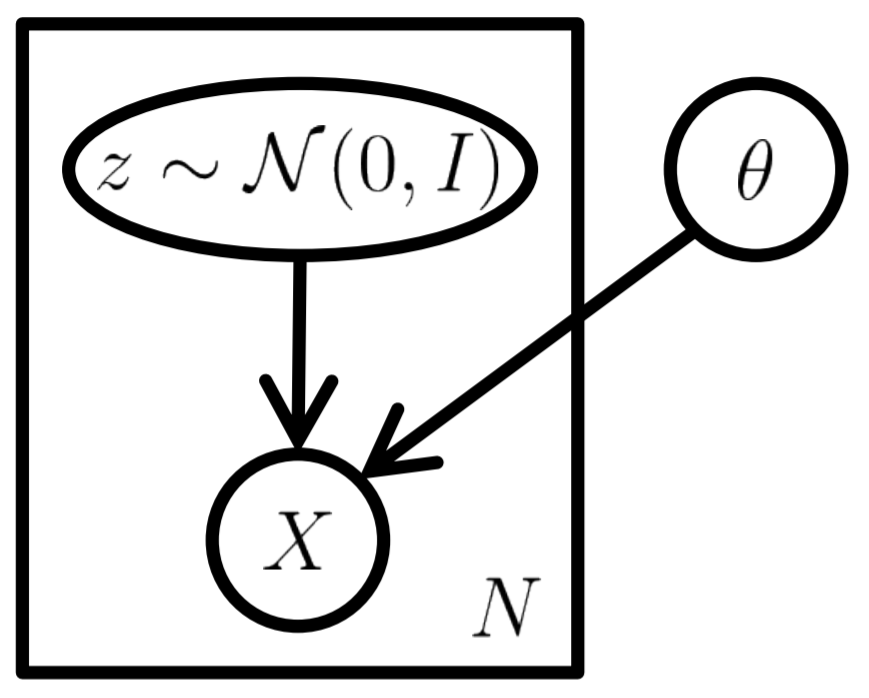
\includegraphics[width=6cm]{./images/vae_model.png}
\caption{VAE的图模型,图片来自于\cite{doersch2016tutorial}}
\label{fig:sample}
\end{figure}

公式化的话,VAE期望优化训练集中的每一个数据点的概率值,$P(X) = \int P(X | z; \theta) P(z) dz$,其中由z生成X的分布是由$\theta$参数化的神经网络。为方便后续推导,我们假定 $P(X | z; \theta) = N(X | f(z; \theta), \sigma^2 \* I)$。图1给出了VAE的图模型,对每一个训练集中的数据点$X$,由$\theta$参数化的神经网络将一个从正太分布中采样出的隐变量$z$映射到$X$。如果直接对上式采样,将意味着很大的计算负担,并且对于大多数的$z$,$P(X|z)$都接近于$0$,很多样本是无意义的。因此,变分自编码器需要另一个函数$Q(z|X)$来拟合真实的$P(z|X)$分布,这也正是名字中变分一词的来历。其中$Q$分布通常也假定为正态分布,由另一个模型估计出来。这样,通过观察下式

\begin{equation}
	\begin{aligned}
		KL(Q(z|X) ||P(z|X)) &= E_{z \sim Q}[\log Q(z|X) - \log P(z | X)] \\
		&= E_{z \sim Q}[\log Q(z|X) - \log P(X | z) - \log P(z)] + \log P(X) \\
	\end{aligned}
\end{equation}

我们移项得到

\begin{equation}
	\begin{aligned}
		\log P(X) &= E_{z \sim Q}[\log P(X|z)] - KL(Q(z|X) | P(z)) + KL(Q(z|X) || P(z|X)) \\
		&\geq E_{z \sim Q}[\log P(X|z)] - KL(Q(z|X) | P(z))
	\end{aligned}
\end{equation}

上式左边正是我们想要优化的:最大化训练集的概率。而上式右边两项又可以通过神经网络求出:两项分别代表重构图片的概率,在高斯假定的情况下近似为L2误差,和两个正态分布之间的KL散度。我们通过优化右边这个变分下界,来近似的最大化训练集的概率。

从表示学习(representation learning)的角度看,VAE学习到了高维空间图像的一个低维表示。在表示学习中,一个重要的任务是学习到一个分离(disentangle)的表示,这种表示既存储了高维空间向量的全部信息,本身又有很强的可解释性。例如对于手写字符图像任务,一种可行的分离表示可以是$n$维隐变量的第一个维度表示字符的类别,第二/三个表示字符的斜度/粗细,每一个维度表征数据集中变化的一个因子(factor of variation)。这种表示意味着我们可以通过调整一个维度来调整生成图像的某一个特征,对风格迁移任务有很大的帮助。在传统的VAE基础之上,研究者提出了不同的VAE变种来提升VAE编码的分离能力,如\cite{Burgess2018UnderstandingDI, RubSchTol18b}。他们可以看作在传统的VAE基础上加入$\int Q(z|X) P(X) dX$,用不同的方式实现这个后验分布,优化模型的分离能力。

上述的分离学习方法专注于在隐变量的每一个维度都分离的控制不同的变化因子。在细粒度的分离学习之外,我们也可以将VAE的隐变量分成几组,每组控制到不同的特征。\cite{vunet2018}文认为图像是由形状(shape)和外表(appearance)共同控制生成,文中提出了一个条件的U-Net,用形状和RGB图片生成新的图片。\cite{Wu2019DisentanglingCA}文用无监督的方法分离图像中的结构和风格信息。本文同样以VAE为理论基础,专注于分离图片中几何信息和风格信息。我们在理论推导方面受到了上两文的启发,但本文选取了深度图表示结构信息,而不是隐变量\cite{vunet2018}或关键点\cite{Wu2019DisentanglingCA},另外在模型实现方面也和上两文有所不同。此外,应对材质迁移后的图片训练集中无监督的情况,我们引入了生成对抗网络来优化生成结果,这些在本章的下一节中会详细论述。

\section{生成对抗网络}

生成对抗网络(GAN)\cite{NIPS2014_5423}是另一种常用的生成模型,与VAE不同,它并不直接估计数据的概率分布,而是间接的近似$P(X)$。GAN的模型分成两个部分:生成器和判别器,前者能采样出和训练集数据同分布的样本,而判别器能够判别一个给定样本是否来自于训练集的分布,二者通常是以神经网络参数化的模型。GAN的训练通过上述两方的博弈,最终得到一个纳什均衡,即生成器不能通过微调参数生成更加以假乱真的图片,判别器也不能通过微调参数提升自己判别真假的能力。和VAE相比,GAN的优化目标并没有用到变分下界,并且神经网络的优秀拟合能力使得GAN理论上是能够拟合任何分布的。另外,由于GAN的优化目标是判断训练集的分布和生成器生成的分布是否拟合,对每一个样本从整体上判断生成质量,经验上它所生成的样本往往更具真实性。而VAE由于损失函数中的重构损失往往由L1/2损失函数估计,这种像素级别的损失函数偏向于生成一个平均图像,导致生成图像往往边界不清晰,图像模糊。

\begin{figure}
\centering
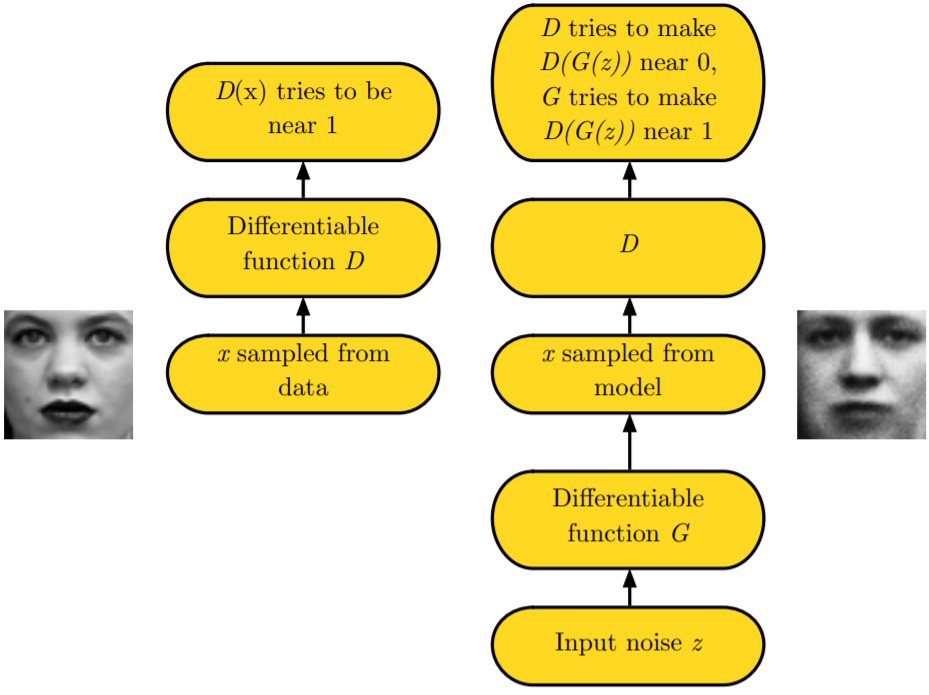
\includegraphics[width=9cm]{./images/gan_model.png}
\caption{GAN的框架,图片来自于\cite{goodfellow2016tutorial}}
\label{fig:sample}
\end{figure}

公式化论述的话,我们遵从GAN原文的记法,训练集$x \sim p_{data}(x)$,生成器和判别器分别记为$G, D$,是两个神经网络,前者接受一个随机变量$z$作为输入,它通常来自一个标准正态分布,力图输出符合分布$p_{data}$的样本,后者类似一个分类器,接受一个样本,输出$[0, 1]$之间的数值,力图对训练集中样本输出1,而对生成器生成的样本输出0。按前文的说明,GAN要优化的是下式

\begin{equation}
	\min_{G} \max_{D} V(D, G) = E_{x \sim p_{data}(x)}[\log D(x)] + E_{z \sim p_{z}(z)}[\log (1 - D(G(z)))]
\end{equation}

GAN原文中证明了上式事实上等价于优化生成器的分布和训练集的Jensen-Shannon散度,亦即对称的KL散度,并且也在理论上论述了最优解的存在性。


在材质迁移的任务中,由于融合了两张图像的材质和内容的图像不可得,因而无法使用L1/2损失函数,在这种情况下,往往使用GAN来判断生成图片的质量。而仅仅判断要求生成图片属于训练集的分布是不足以要求生成图片融合了不同的风格和内容的。一种可行的改进是使用判别器接受成对的图片判别是否拥有同一材质或内容\cite{ma2017pose},这要求合理的利用训练数据构造真和假的数据对。图像生成任务中,另一种对生成对抗网络的改进是使用多尺度的判别器,这种方法利用多个判别器分别接受原尺度和按不同比例缩小的图片,使得生成图片在各个尺度上都能拟合训练集的特征。利用ProGAN\cite{Karras2017ProgressiveGO}的角度来看,我们也可以认为多尺度的判别器事实上为生成器提供了更多的信息,使得它能够从小尺度(也就是全局)的特征开始学习,最后去拟合大尺度(细节)的特征。本文的方法使用了上述两种对生成对抗网络的改进,使生成图像更加真实。

\section{本文实验原理}

我们首先正式的阐述本文研究的问题,并且明确后文中会用到的记号。三维模型的最优视图生成任务即针对一个给定的三维模型$m \in M$,我们的模型能够生成一张图片$i \in I = R^{m \times n \times 3}$,在后文中除非特殊说明$m = n = 128$。我们将这个任务拆解为给定一个视角$v$,将三维模型投影为深度图和给定一个材质$s$,将深度图渲染为RGB图片的两个问题,如(2.4)式。其中$proj(.)$为投影函数,它能够给定一个三维模型和视角,生成一个深度图,即每一个像素的取值和模型上对应的点距相机的距离有关的图片。我们实验中的视角模型只考虑方位角(az)、仰角(el)的变化,其他的参数都预设为Blender中的默认值。

\begin{equation}
	\begin{aligned}
		i_{d} &= proj(m, v) \in R^{m \times n}, vp = [az, el, dist] \\
		i_{out} &= f(i_{d}, s)
	\end{aligned}
\end{equation}
(2.4)式确定的两个问题,前者可以确定性的通过Blender渲染,关于视角选择的问题会在后文中阐述。而后者我们应用了VAE和GAN来指导生成,在这里我们假定每一张RGB图片$i \in I = R^{m \times n \times 3}$都由内容(c)、材质(s)和视角(v)三个独立的变量指导生成,其中内容和材质是需要推断的隐变量,而视角在训练时给出,是已知的变量。而每一张深度图$i_{d} \in R^{m \times n}$只由内容和视角两个互相独立的变量指导生成,而视角信息在训练时给出,因此可以粗略的认为深度图表征内容信息。公式化表示的话:

\begin{equation}
	i_{RGB} \sim P(i | c, s, v), i_{d} \sim P(i | c, v)
\end{equation}

我们训练时先从真实图片中提取出内容和材质隐变量,再通过这两个隐变量重组出输出图片。类似前文对VAE的推导,我们得到训练过程中优化训练集的概率,如(2.6)式。其中第一、四步推导应用了贝叶斯公式,第二步的推导基于我们对材质隐变量的高斯分布假设$p(c | i) = N(f(i, \theta), I)$,因而$-\log p(c | i) = \frac{1}{2}||c - f(i, \theta) ||^2 + \frac{N}{2}\log (2\pi) \geq 0$,第三步利用对数函数的凸性,是在积分意义下的Jensen不等式。

\begin{equation}
	\begin{aligned}
		\log p(i) &= \log p(c) + \log p(i | c) - \log p(c | i) \\
		&\geq \log p(c) + \log  \int p(i, s | c) ds \\
		&\geq \log p(c) + E_{q} \log \frac{p(i, s | c)}{q(s | i, c)} \\
		&= \log p(c) + E_{q} \log \frac{p(i | c, s)p(s)}{q(s | i)} \\
		&= \log p(c) + E_{q} \log p(i | c, s) + KL(q(s) || p(s)) \\
	\end{aligned}
\end{equation}

参考CVAE的推导,两边同时对视角取条件,得到最终的优化目标

\begin{equation}
	\log p(i | v)= \log p(c) + E_{q} \log p(i | c, s, v) + KL(q(s) || p(s))
\end{equation}

其中第一项代表我们推导出的内容隐变量的概率,它越表征内容信息,这个概率值应越大,在实验中我们通过网络重构出的深度图和真实深度图之间的L1损失衡量,注意与\cite{Wu2019DisentanglingCA}提出的在关键点上的弱监督不同,我们在这里加的是一个很强的限制条件。第二项即为重构出的图片的真实性,我们遵从VAE的惯例,用重构出的图片和输入图片之间的L1损失实现。第三项为推导出的材质隐变量的KL散度损失,用两个正态分布之间的KL散度实现。

\begin{figure}
\centering
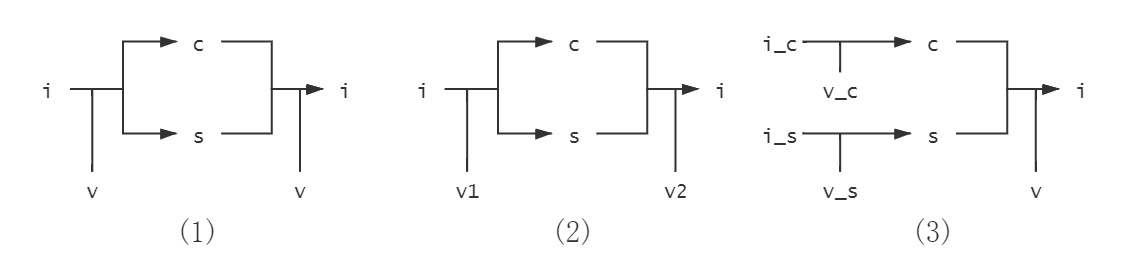
\includegraphics[width=15cm]{./images/my_model.png}
\caption{我们设计的三个实验的流程}
\label{fig:sample}
\end{figure}

上述损失函数只描述了重构图片时的损失,单独实现这三个损失函数只保证了我们模型重构图片和采样的精度,但并不能保证我们假定的隐变量之间互相独立。为此,除了图像重构之外,我们另外设计了两个实验:新视角生成和材质迁移。三个实验的流程见图3。注意视角变量$v$在训练时给出,我们在从图片中提取出材质和内容变量的过程中也输入已知的视角信息,来提升提取信息的准确性。这种做法也有助于提取到视角无关的材质和内容信息。

为保证视角和其他隐变量相互独立,我们在训练过程中给出所有图片的视角,并且设计了新视角生成的实验:从输入图片中提取内容和材质隐变量,在另一个视角下生成输出图片。在这个实验中,视角$v^{1}, v^{2}​$均在训练时给出,损失函数的推导同上,损失函数的实现也完全相同。

为保证内容和材质变量相独立,我们设计了交换材质迁移的实验。在这个实验中,材质和内容隐变量分别从不同的图片中提取出,融合得到生成的图片。我们希望生成的图片能够兼具两张图片的内容和材质。但和之前叙述过的实验不同,这个实验并没有监督数据,因此不能用L1/2损失来估计优化目标中$E_{q} \log p(i | c, s, v)$一项,在这里我们应用生成对抗网络来估计这一项。如前文叙述,生成对抗网络的损失函数只在分布的意义上要求生成图片属于训练集的图片的分布,这个损失函数本身只要求生成图片的真实性,并没有要求生成图片融合两张图片的内容和材质。但在实验中,我们发现只应用这个损失函数,生成的图片也足以达成这个目标。为更进一步要求这个目标,我们在训练时加入另一个判别器,它接受两张图片作为输入,判别这两张图片是否具有同一材质。对内容隐变量不需加入这个约束项,因为作为输入的深度图本身编码了足够多的内容信息也有L1/2损失函数约束,然而材质信息是形式上没有其他约束的。

在输入一张图片能够生成多视角下视图的基础上,我们讨论最优视角选择的问题。遵循以往研究的假设,我们认为三维模型的最优视角是包含最多信息的视角。但不同于以往直接在三维模型或是二位视图上定义并计算信息,我们采用重构其他视图的误差作为信息的衡量。一个包含更多信息的视角应当能够更加准确的重构其他视角下的信息,例如对于汽车而言包含车头和车尾的视角比侧面的视角会包含更多的信息。公式化表达的话,我们根据以下公式选取最优视角,其中$m$代表三维模型,$f(i_{vp}, vp, vp')$表示输入$vp$视角下的视图,生成$vp'$视角下的视图的函数。

\begin{equation}
	vp_{best} = \mbox{argmin} E_{m, vp'} | i_{vp'} - f(i_{vp}, vp, vp')|
\end{equation}


通过对三维模型$m$和视角$vp'$取期望,我们得到平均意义下包含信息最多的视角。注意,在这里的$i_{vp}$是渲染好的包含材质的图片而不是深度图或是轮廓图。这意味着与之前的方法不同,我们讨论的最优视图是包含材质的三维模型的最优视图。

\section{模型实现细节}

本节将讨论我们的方法的具体实现,包括各个模型的输入输出、参数设置和训练过程。上一节的讨论可以得到我们需要实现的映射包括

\begin{equation}
	c = f(i, v),\ i_d = g(c, v), s = h(i ,v), i = m(c, s, v)
\end{equation}

以及为保证对抗训练的判别器,下文中会依次详细的介绍每一部分的实现和参数,以及我们应用到的两个模块SPADE\cite{park2019SPADE}和CoordConv\cite{NIPS2018_8169}的细节。我们的代码参考了Pix2Pix-CycleGAN\footnote{https://github.com/junyanz/pytorch-CycleGAN-and-pix2pix},SPADE\footnote{https://github.com/NVlabs/SPADE},CoordConv\footnote{https://github.com/walsvid/CoordConv}的实现细节,在整合这些模块的基础上编写了自己的模型和训练代码,实现细节开源在Github上\footnote{https://github.com/DanDoge/FYP}。后文中我们会使用形如图4的图来描述我们的模型的具体结构,其中每一层的含义和参数意义与它们在pytorch\cite{NEURIPS2019_9015}中的定义一致,如$conv(inputnc=1, outputnc=3, kernelsize=3, stride=1, padding=1)$代表输入一通道、输出三通道、卷积核大小$3 \times 3$、步长为$1$、外衬一像素的卷积层。

\subsection{生成器}

我们将生成深度图像和RGB图像的任务都用相似结构的生成器实现。我们认为给定视角和内容隐变量,深度图可以被唯一的确定,因此生成RGB图片的任务可以重新叙述为$i = m(c, s, v) = m'(i_d, s)$。因为深度图$i_d = g(c, v)$中包含了渲染图片必须的视角和内容信息,因此用只接受深度图作为输入的$m'$函数来近似接受隐变量的$m$函数是可以做到的,实验中我们发现这一近似提升了生成结果。类似的,生成深度图的任务也表示为$i_{d} = g(f(i, v_1), v_2)$。在这样的表示下,生成RGB图片的任务和生成深度图的任务具有一定的对称性,可以利用同样结构的网络实现,也便于利用已有的图片到图片翻译的工作的成果。下文中我们只讨论形如$y = f(x, b)$形式的生成任务。我们借鉴已有的图像到图像翻译工作成果,将$f(.)$函数用编码器-解码器的结构实现,编码器用来从输入变量中提取对生成有用的信息,解码器用来将这些信息整合,生成最终期望的图像。

\begin{figure}
\centering
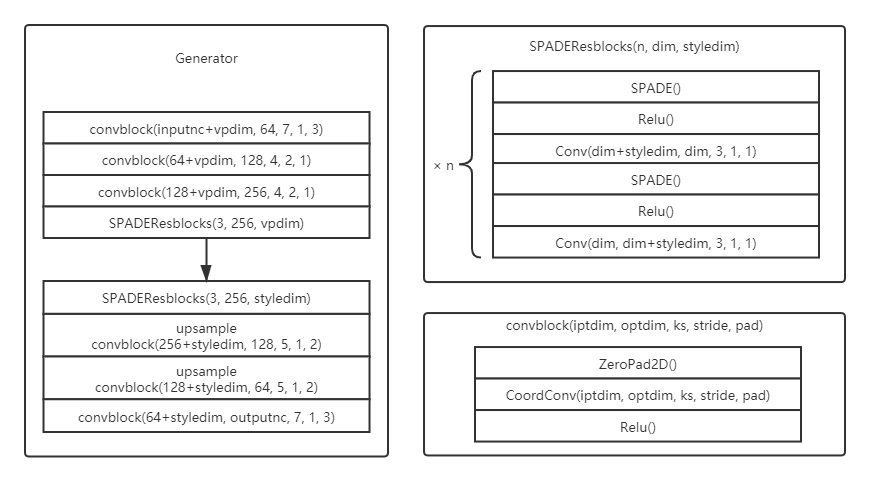
\includegraphics[width=15cm]{./images/generator.png}
\caption{生成器的框架}
\label{fig:sample}
\end{figure}


编码器用连续的卷积模块和残差模块组成,前者通过步长为2的卷积下采样,精炼输入中的信息,后者通过预测一个增量信息,精修卷积模块提取出来的信息。此外,在每一层我们都输入视角信息辅助生成,我们将视角信息作为两个通道的变量附加到每个模块的输入中。对于两个任务,这都有助于辅助编码器生成和视角无关的信息,对生成深度图的任务这是必须加入的。我们期望编码器能够从二维图像中提取出三维信息,并且通过解码器将三维信息映射回二维平面。对此,二维图像中的坐标信息是十分重要的,例如输入一辆车的侧面时,有关车轮的信息更有可能在图像的下面获取到而不是上面,解码三维信息时也同理。而卷积层由于自身的空间不变性并不能实现这种需求。为解决这种矛盾,我们将生成器中的所有卷积层替换成坐标卷积(coordconv),这种卷积现在输入变量后附加两个通道,分别包含每一个位置的x,y坐标,显式的让卷积层获得位置信息,在不同位置生成不同的输出特征。

解码器是近似对称的结构,对于编码器提取出的信息,先经过几个残差模块,再通过上采样和卷积模块还原到输入的分辨率。在解码器整合内容信息和材质信息时,我们采用了SPADE模块来帮助生成。我们采用的SPADE模块由InstanceNorm和一个MLP组成,MLP负责从深度图和材质特征中估计出用来正则化特征的$\gamma$和$\beta$。通过将输入特征的均值和方差替换成估计出的统计量,我们试图在特征维度对齐生成图片的分布和训练图片的分布。不同的SAPDE模块MLP参数不同,这样我们就能利用连续的几个SAPDE模块逐渐将材质信息和内容信息整合。在实验过程中,我们尝试过SPADE以外的其他方法,例如将特征直接拼接在每层的末尾、利用Unet生成,但结果不如SPADE的效果好。

根据两个生成任务不同的特性,我们采用了不同的超参数。生成深度图的任务要求编码器提取到更加全局的信息,掌握三维模型的结构,以便解码时能够生成不同视角下的深度图,因此对这个任务下采样次数设置为4,而生成RGB图片的任务只设定为2。为平衡两个模型的复杂性以便训练稳定,生成RGB图片的生成器通道数加倍,这也符合渲染任务本身的复杂性。


\subsection{编码器}

\begin{figure}
\centering
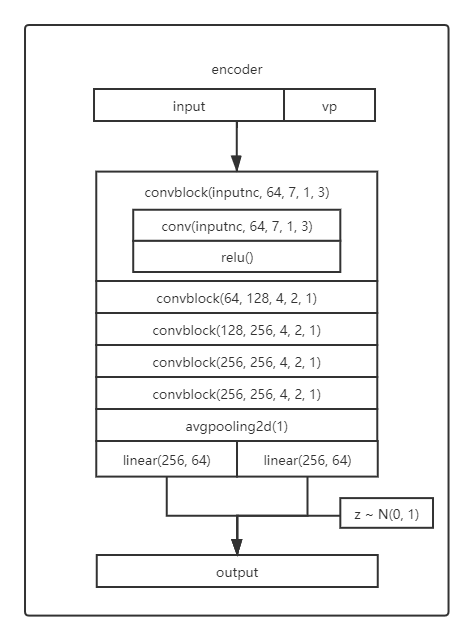
\includegraphics[width=10cm]{./images/encoder.png}
\caption{编码器的框架}
\label{fig:sample}
\end{figure}

编码器用来实现$s = h(i, v)$,从图像中提取出和视角无关的材质特征。编码器在几个卷积模块和全局池化层之后,利用两个全连接层估计材质隐变量的均值和方差。其中一个卷积模块由coordconv和激活层组合而成,全局平均池化层将各个位置提取到的材质信息整合成全局的材质特征。在我们的实验中,材质隐变量的维度设定为64维,这足以表征材质信息。视角信息只在最开始拼接在图像上,使得输入编码器的变量通道数为$3 + 2 = 5$维。

\subsection{判别器}

判别器采用卷积层和非线性层叠加的方式实现。每一次卷积都使用步长为$2$的卷积,并且倍增输出的通道数以实现在下采样的同时,不丢失原图中信息的效果,通道数最大值设定为$1032$。最后一层卷积输出一通道的结果,判别输入向量的真实性。在我们的实验中,下采样的次数为$4$次,对于输入的$128 \times 128$的图像最终输出长宽为$8\times8$的向量,每一个位置表示它所对应的原图中$16\times16$的部分的真实性。对于后文会叙述的一次输入两张图片的情况,每一个位置表示它对应的$16\times16$的部分的两张图片是否属于同一个材质。在原尺度的判别器之外,我们还增加了一个小尺度的判别器,它的输入是原尺度判别器输入$\frac{1}{2}$下采样一次的结果。它的网络结构与原尺度判别器类似,只是通道数减半,以保证每一个通道的信息量大致和原尺度相同。它的输出的每一个位置同样对应它的输入的$16\times16$的部分,也就是原图的$32\times32$的部分。加入小尺度的判别器保证了输出图像在多尺度上都和目标图像有相同的统计特征,为生成器提供更多的指导。优化过程中我们对两个尺度的判别器的输出都做同样的优化:对真样本。下文中提到的判别器都指的是原尺度和小尺度判别器的组合,图中显示了两个尺度的判别器组合的网络结构。

判别器的损失函数采用最小二乘优化(LSGAN),原文中证明了它等价于优化皮尔森卡方散度,训练更加稳定。我们尝试了其他GAN损失函数的变体,包括WGAN,对生成图像的结果没有很大影响。判别器的损失函数优化目标是使得生成器的生成结果贴近于某一个分布,而这一个分布是通过训练数据指定的。不同的训练目标对应着不同的指导分布,也就对应着不同的输入数据。在我们的训练过程中,我们希望生成器的生成结果达到下列两个目标:

\begin{itemize}
	\item 生成高质量的图片。为此我们使用生成图片和真实图片分别作为假/真数据的代表输入判别器,这个损失函数使得生成图片能更具真实性。
	\item 生成具有特定材质/内容的图片。为此我们引入另一种判别器,它的输入是两张图片的拼接,即输入通道数加倍。训练时,对于RGB图片的生成任务,我们要求生成图片的材质相同,采用同一个物体在不同视角下的RGB图片作为真样本,用生成器输出的结果和一张真实图片拼接作为假样本训练;对于深度图的生成任务,我们对称的引入一个要求生成深度图的内容一致的判别器。
\end{itemize}

所以我们的网络中共有八个判别器,分别对应两个生成任务、两个目标和两种尺度的组合。

\begin{figure}
\centering
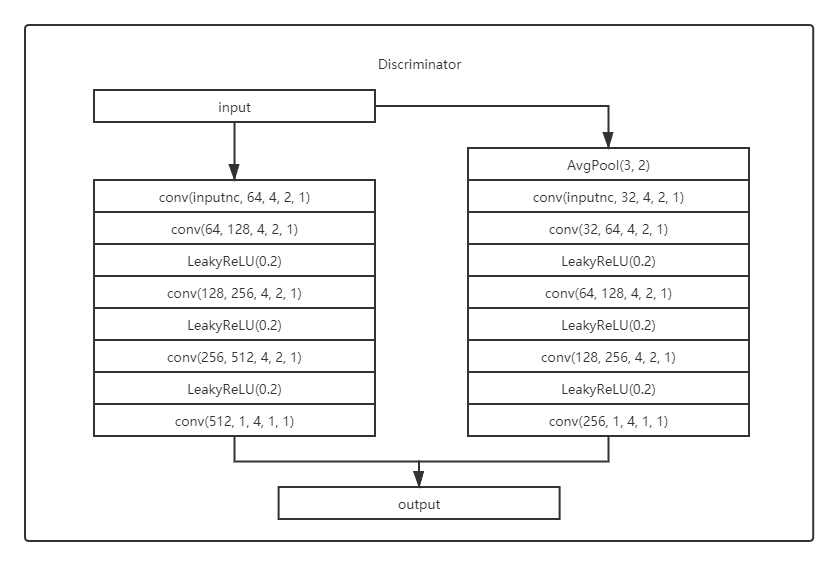
\includegraphics[width=15cm]{./images/discriminator.png}
\caption{判别器的框架}
\label{fig:sample}
\end{figure}

生成对抗网络的训练不稳定,可能在训练过程中出现网络崩溃的现象,这往往是判别器学习过快导致的。对此kato文在新视角生成任务种采用了一种弱化的判别器:即将原视角下重建的结果作为真样本,新视角下生成的结果作为假样本。这样做的初衷是训练初期重建的结果往往会好过新视角生成的结果,判别器能够学习到一些知识,但又不至于学习的过快。我们尝试过这种训练方式,但结果并不好。因为这样判别器学习到的分布特征其实完全来自于生成器,整个网络的监督信息依赖于对生成结果的L1/2损失函数。在我们的实验中,单独这个损失函数是不足够的,因此我们的训练过程完全采用真实图片输入。



\clearpage

\chapter{实验结果}

\section{数据集的构成}

为了公平比较,我们使用了与\cite{Zhou2016ViewSB}相同的数据集进行实验,这个数据集也是后续新视角生成任务公用的数据集。\cite{Zhou2016ViewSB}文将shapenet-car分支下的模型分成两部分,分别作为训练集和测试集,训练集有5997个模型,测试集有1500个模型。按新视角生成任务的惯例,对每一个模型在54个视角下渲染,分别是方位角0递增到340,步长为20,仰角分别取0,10,20。我们使用Blender的python脚本先渲染出这些视角下的深度图和RGB图片,以减少训练时渲染的时间开销。\cite{Zhou2016ViewSB}和\cite{Su2015MultiviewCN}开源的代码中采用了自己的渲染器,为保证实验结果的公平性,这些方法都是在我们渲染出的数据集上实验。对于真实数据,我们采用\cite{6755945}中提出的汽车数据集,其中分别包含8144和8401张训练和测试的汽车图片。因为我们的模型并没有编码背景的能力,我们用预训练的场景分割算法DeepLabv3(引文)分割出包含汽车的部分。为保证真实图片的数据分布和我们的合成图片尽可能的贴合,我们删去了物体大小过小,和物体不居中的图像。

\section{视角生成任务}

为衡量我们方法中分离内容与材质特征的部分的有效性,下面展示我们的方法和其他没有分离特征的新视角生成的方法比较的结果。我们用L1误差和FID来比较各个方法的结果,其中前者用每个像素位置的平均误差度量生成图片的准确性,后者用生成图片和真实图片这两个分布的距离度量生成图片的真实性。我们用新视角生成中两个经典的算法\cite{Zhou2016ViewSB}和\cite{TDB16a}作为比较标准,前者作为流模型的代表,后者做为作为直接生成像素方法的代表。遵循新视角生成任务测试的惯例,我们从测试集中随机选取出10k张图片计算L1损失和FID。观察到,我们的方法在生成图片准确性和真实性上都和新视角生成方法具有可比性。这说明我们的分离内容与材质的生成模式是有效的,隐变量的分离并不以生成图片的质量为代价,反而增强了生成图片的质量。我们在表中同样列出了我们使用的各个训练技巧的之后的结果。【】图中展示了我们的算法在连续变换视角的条件下的生成结果,模型有能力提取到与视角无关的内容信息,并用于生成各个视角下的视图。

一个表,两张图

\section{材质迁移任务}

分离隐变量中的材质部分和内容部分也使得我们的模型能够实现材质迁移的效果:即生成融合两张图片的材质和内容特征的视图,这是新视角生成方法所不能做到的。我们在下面展示材质迁移的结果。可以看到我们的算法能够迁移基本的色彩信息,同时完美的保留内容图片的内容结构。观察到生成结果在细节方面有一些不足之处,在后文中会详细讨论其原因。【】图中展示了插值实验的结果,我们对最左端和最右端的图片提取到的材质变量进行插值,生成中间的各个图像。实验结果表明了模型能够学习到连续的材质隐变量流形,也即我们对材质变量的高斯分布假设是有效的。

我们从材质隐变量的分布中随机采样,结果如图【】。

两张图,FID数据

\section{最优视角选择}

我们认为最优视角是在考虑了材质的条件下包含最多信息的视角,具体的计算方法在理论一节中有详细叙述。和以往几何学的方法不同,我们的方法直接在RGB图片的尺度上选择最优视角。这种方法即考虑到材质信息,也没有忽略掉模型的几何结构的影响:我们观察到几何结构复杂的地方通常也是材质信息高频的区域。定性试验上,我们和\cite{Dutagaci2010ABF}文中列出的表现较好的方法\cite{Vzquez2003AutomaticVS}和\cite{Lee2005MeshS}进行了比较,前者在二维视图上定义信息,后者在三维模型上定义信息。为保证公平性,两种方法也是从上文定义的54个视角中选取最优视角。我们参考原文的描述和开源的方法复现了这两种方法,在测试集上的定性结果在图【】中。Mesh Saliency\cite{Lee2005MeshS}因为倾向于选择能看到模型几何上更加复杂的区域的视图,它在汽车数据集上倾向于选择侧面的视角,没有很好的把握住模型上材质高频变化的区域。



作为补充,为说明利用模型生成结果定义最优视角的方式是有意义的,我们展示了在不同的输入和输出视角下重构图片的误差大小。下图中横轴代表输入视角、纵轴代表输出视角。我们观察到输出视角对重构图片的误差影响很小,而输入视角几乎决定了生成图片的误差大小。我们认为这是因为我们提取模型视角无关的内容和材质信息的结构产生了这个结果。对于包含更多细节的视角,例如包含车头或车尾的视角,模型能够提取到更多更完整的内容和材质信息,因此在多视角下都能够重构出更好的视图,反之则在各个视角下重构结果都变差。因此可以通过重构误差来反推出视角包含信息的多少。相反,基于流的生成方法,生成图片的误差取决于输入输出视角之间的差距,不能够用生成图片的期望误差来评判输入视角的好坏。

两张图

\section{真实图片输入}

下面我们展示我们的模型在真实图片上的结果。在合成数据集上训练的模型,不能有效的提取出真实图片中的材质信息,因此我们用真实图片的一部分精修训练好的模型,再在测试集上面测试。同时,应用视角估计的结果,我们可以将真实图片的视角和材质都迁移到深度图上,结果如图【】。

两张图

\clearpage

\chapter{总结与展望}

生成三维模型的最优视图会增强人们对三维模型的理解,便利三维模型的检索和可视化,是一个具有研究价值和使用价值的问题。本文回顾了以往在生成最优视图领域的工作,提出了一个新的模型用于生成三维模型的视图,并提出了一个选择最优视角的方法。在详细描述方法原理之后,我们通过和以往方法的比较,证明了我们提出的方法的有效性。它和以往的新视角生成算法效果相当,并且能够实现图片领域的材质迁移,也能通过一些精修应用到真实图片上。基于这种方法定义的选择最优视角的算法也能够选取出材质意义上更加优秀的算法。

在上文介绍过的模型优点之外,我们的方法还有以下不足:材质提取只停留在全局层面,对于细节特征并不能很好的还原。这是本文采用的卷据网络提取特征,并且像素级别生成的通病。我们观察到对于材质多样的模型,我们的方法只能迁移其中主要的或者平均的材质;而对于细粒度的特征,例如车头车尾的细节,我们的模型倾向于生成数据集中平均的特征。这可能是因为
\begin{itemize}
	\item 细粒度的特征只停留到卷积网络,深层的特征只留下全局的特征,
	\item 像素级别的生成网络的损失函数倾向于生成平均特征,这在VAE一节中有详细的讨论。
\end{itemize}
相反的,利用流的模型能够较好的保留原图中的细节特征。将材质和内容相分离的思想应用到流生成模型上可能是一个有趣的未来工作。

另外我们的工作只是在图像层面能够重建三维模型的材质信息,进一步的工作可能是利用我们对深度图的上色结果给三维模型的面上色,如何根据这一目标修改模型结构,并有效的整合多视角下的上色结果也是未来的一个工作方向。





\clearpage


\addcontentsline{toc}{chapter}{参考文献}
\fancypagestyle{plain}
{
	\fancyhf{}
	\fancyhead[RE,RO]{参考文献}
	\fancyhead[LE,LO]{北京大学本科生毕业论文}
	\fancyfoot[CO,CE]{~\thepage~}
	\renewcommand{\headrulewidth}{0.7pt}
	\renewcommand{\footrulewidth}{0pt}
}
\fancyhf{}
\fancyhead[RE,RO]{参考文献}
\fancyhead[LE,LO]{北京大学本科生毕业论文}
\fancyfoot[CO,CE]{~\thepage~}
\renewcommand{\headrulewidth}{0.7pt}
\renewcommand{\footrulewidth}{0pt}






\bibliographystyle{unsrt}
\bibliography{ref}
\clearpage





\linespread{1}\selectfont
\normalsize
%小四号,中文宋体,英文Time new roman,1倍行距
\chapter*{本科期间的主要工作和成果}

\noindent 本科期间参加的主要科研项目

\noindent 本研基金
\begin{enumerate}
	\item 国家创新训练计划. 基金类型. 连宙辉. 2018-2019
\end{enumerate}



\addcontentsline{toc}{chapter}{本科期间的主要工作和成果}
\fancypagestyle{plain}
{
	\fancyhf{}
	\fancyhead[RE,RO]{本科期间的主要工作和成果}
	\fancyhead[LE,LO]{北京大学本科生毕业论文}
	\fancyfoot[CO,CE]{~\thepage~}
	\renewcommand{\headrulewidth}{0.7pt}
	\renewcommand{\footrulewidth}{0pt}
}
\fancyhf{}
\fancyhead[RE,RO]{本科期间的主要工作和成果}
\fancyhead[LE,LO]{北京大学本科生毕业论文}
\fancyfoot[CO,CE]{~\thepage~}
\renewcommand{\headrulewidth}{0.7pt}
\renewcommand{\footrulewidth}{0pt}
\clearpage





\linespread{1.5}\selectfont
\normalsize
\chapter*{致谢}

感谢

\addcontentsline{toc}{chapter}{致谢}
\fancypagestyle{plain}
{
	\fancyhf{}
	\fancyhead[RE,RO]{致谢}
	\fancyhead[LE,LO]{北京大学本科生毕业论文}
	\fancyfoot[CO,CE]{~\thepage~}
	\renewcommand{\headrulewidth}{0.7pt}
	\renewcommand{\footrulewidth}{0pt}
}
\fancyhf{}
\fancyhead[RE,RO]{致谢}
\fancyhead[LE,LO]{北京大学本科生毕业论文}
\fancyfoot[CO,CE]{~\thepage~}
\renewcommand{\headrulewidth}{0.7pt}
\renewcommand{\footrulewidth}{0pt}





\end{document}
